\documentclass[11pt,]{article}
\usepackage{lmodern}
\usepackage{amssymb,amsmath}
\usepackage{ifxetex,ifluatex}
\usepackage{fixltx2e} % provides \textsubscript
\ifnum 0\ifxetex 1\fi\ifluatex 1\fi=0 % if pdftex
  \usepackage[T1]{fontenc}
  \usepackage[utf8]{inputenc}
\else % if luatex or xelatex
  \ifxetex
    \usepackage{mathspec}
  \else
    \usepackage{fontspec}
  \fi
  \defaultfontfeatures{Ligatures=TeX,Scale=MatchLowercase}
\fi
% use upquote if available, for straight quotes in verbatim environments
\IfFileExists{upquote.sty}{\usepackage{upquote}}{}
% use microtype if available
\IfFileExists{microtype.sty}{%
\usepackage{microtype}
\UseMicrotypeSet[protrusion]{basicmath} % disable protrusion for tt fonts
}{}
\usepackage[margin = 1.5in]{geometry}
\usepackage{hyperref}
\PassOptionsToPackage{usenames,dvipsnames}{color} % color is loaded by hyperref
\hypersetup{unicode=true,
            pdftitle={Integration Among US Banks: Rerun},
            pdfauthor={Abhinav Anand and John Cotter},
            colorlinks=true,
            linkcolor=blue,
            citecolor=magenta,
            urlcolor=red,
            breaklinks=true}
\urlstyle{same}  % don't use monospace font for urls
\usepackage{longtable,booktabs}
\usepackage{graphicx,grffile}
\makeatletter
\def\maxwidth{\ifdim\Gin@nat@width>\linewidth\linewidth\else\Gin@nat@width\fi}
\def\maxheight{\ifdim\Gin@nat@height>\textheight\textheight\else\Gin@nat@height\fi}
\makeatother
% Scale images if necessary, so that they will not overflow the page
% margins by default, and it is still possible to overwrite the defaults
% using explicit options in \includegraphics[width, height, ...]{}
\setkeys{Gin}{width=\maxwidth,height=\maxheight,keepaspectratio}
\IfFileExists{parskip.sty}{%
\usepackage{parskip}
}{% else
\setlength{\parindent}{0pt}
\setlength{\parskip}{6pt plus 2pt minus 1pt}
}
\setlength{\emergencystretch}{3em}  % prevent overfull lines
\providecommand{\tightlist}{%
  \setlength{\itemsep}{0pt}\setlength{\parskip}{0pt}}
\setcounter{secnumdepth}{0}
% Redefines (sub)paragraphs to behave more like sections
\ifx\paragraph\undefined\else
\let\oldparagraph\paragraph
\renewcommand{\paragraph}[1]{\oldparagraph{#1}\mbox{}}
\fi
\ifx\subparagraph\undefined\else
\let\oldsubparagraph\subparagraph
\renewcommand{\subparagraph}[1]{\oldsubparagraph{#1}\mbox{}}
\fi

%%% Use protect on footnotes to avoid problems with footnotes in titles
\let\rmarkdownfootnote\footnote%
\def\footnote{\protect\rmarkdownfootnote}

%%% Change title format to be more compact
\usepackage{titling}

% Create subtitle command for use in maketitle
\newcommand{\subtitle}[1]{
  \posttitle{
    \begin{center}\large#1\end{center}
    }
}

\setlength{\droptitle}{-2em}

  \title{Integration Among US Banks: Rerun}
    \pretitle{\vspace{\droptitle}\centering\huge}
  \posttitle{\par}
    \author{Abhinav Anand and John Cotter}
    \preauthor{\centering\large\emph}
  \postauthor{\par}
      \predate{\centering\large\emph}
  \postdate{\par}
    \date{2018/08/18}

\linespread{1.25}
\usepackage{amsmath}

\begin{document}
\maketitle

\section{Median US Bank Integration}\label{median-us-bank-integration}

\begin{center}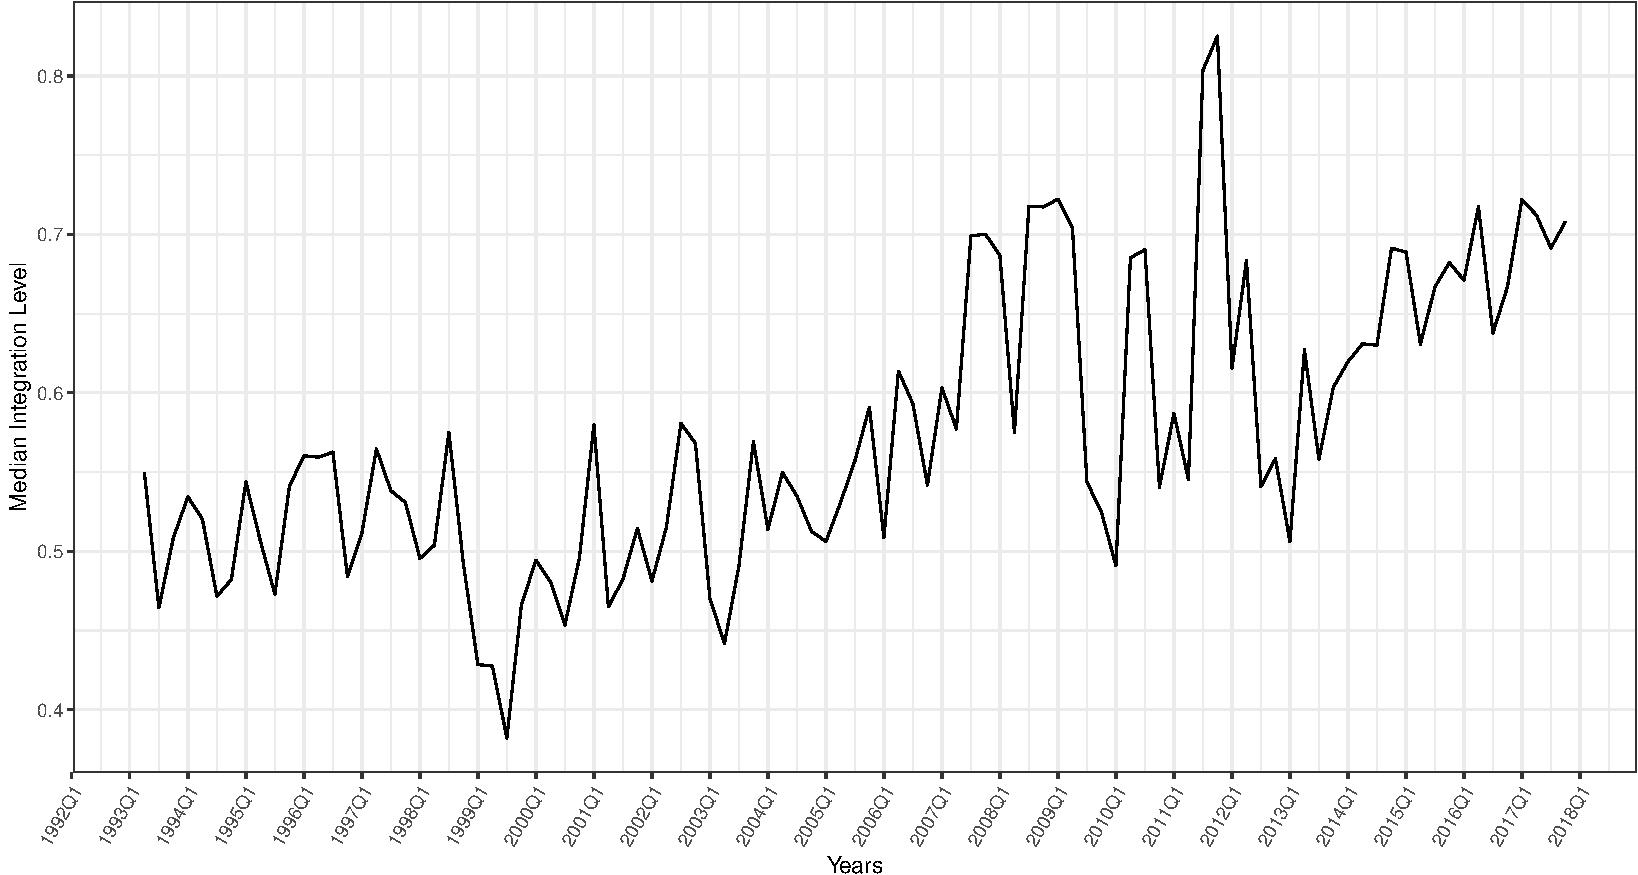
\includegraphics{AC_US_Bank_Int_Results_1_files/figure-latex/med_US_bank_int-1} \end{center}

\section{Empirical Distribution of US Bank
Integration}\label{empirical-distribution-of-us-bank-integration}

\begin{center}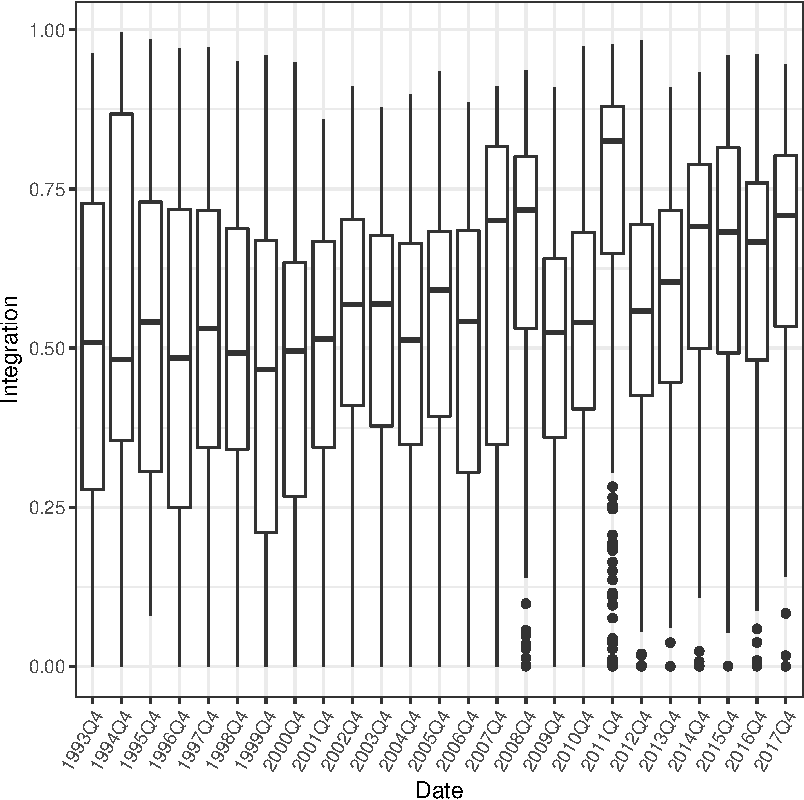
\includegraphics{AC_US_Bank_Int_Results_1_files/figure-latex/emp_distr_US_bank_int-1} \end{center}

\section{Most Integrated Banks}\label{most-integrated-banks}

\begin{longtable}[]{@{}lr@{}}
\toprule
rowname & value\tabularnewline
\midrule
\endhead
FIRST BANCORP INC ME & 0.8940538\tabularnewline
FIRST HORIZON NATIONAL CORP & 0.8902213\tabularnewline
CATHAY GENERAL BANCORP & 0.8722374\tabularnewline
EXECUFIRST BANCORP INC & 0.7785441\tabularnewline
BOSTON PRIVATE FINL HLDGS INC & 0.7719863\tabularnewline
KEYCORP & 0.7588579\tabularnewline
BANKUNITED INC & 0.7564036\tabularnewline
CAPITAL CITY BANK GROUP & 0.7546513\tabularnewline
O F G BANCORP & 0.7408198\tabularnewline
HUNTINGTON BANCSHARES INC & 0.7327105\tabularnewline
FIRST DEFIANCE FINANCIAL CORP & 0.7321722\tabularnewline
OCEANFIRST FINANCIAL CORP & 0.7287170\tabularnewline
AMERISERV FINANCIAL INC & 0.7268199\tabularnewline
NARA BANCORP INC & 0.7249545\tabularnewline
DIME COMMUNITY BANCSHARES & 0.7196594\tabularnewline
EAGLE BANCORP INC & 0.7185455\tabularnewline
MAINSOURCE FINANCIAL GROUP INC & 0.7178897\tabularnewline
BEAR STATE FINANCIAL INC & 0.7115614\tabularnewline
FLUSHING FINANCIAL CORP & 0.7101900\tabularnewline
1ST SOURCE CORP & 0.7080712\tabularnewline
BANK OF THE OZARKS INC & 0.7071273\tabularnewline
NORTHFIELD BANCORP INC DE & 0.7063278\tabularnewline
FRANKLIN FINANCIAL NETWORK INC & 0.7039904\tabularnewline
HAWTHORN BANCSHARES INC & 0.6972166\tabularnewline
BRIDGE BANCORP INC & 0.6969681\tabularnewline
\bottomrule
\end{longtable}

\begin{center}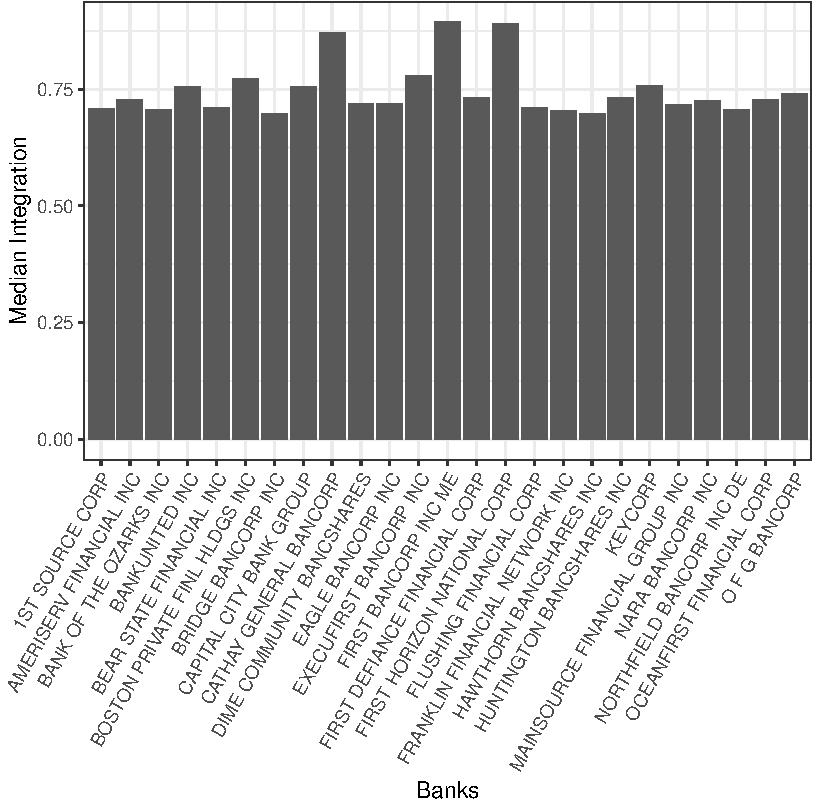
\includegraphics{AC_US_Bank_Int_Results_1_files/figure-latex/most_int-1} \end{center}


\end{document}
